\section[Metodología AG]{Metodología del Algoritmos Genéticos}

\begin{frame}{Anexo \thesection~: Selección de Padres}%
    \vspace{-0.15cm}
    \begin{figure}[H]
        \centering
        \adjustbox{max width=\textwidth, max height=0.7\textheight}{%
            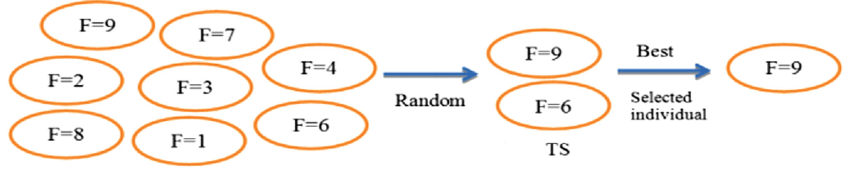
\includegraphics{img/appendixC/tournament-selection.png}
        }
        \vspace{-0.25cm}
        \caption{\tiny~Ilustración que describe el proceso de Selección de padres.~\textit{Adaptado de:}~\cite{ayoub2020}}%
        \label{fig:tournament_selection}
    \end{figure}
\end{frame}

\begin{frame}{Anexo \thesection~: Cruzamiento}%
    \vspace{-0.15cm}
    \begin{figure}[H]
        \centering
        \adjustbox{max width=\textwidth, max height=0.7\textheight}{%
            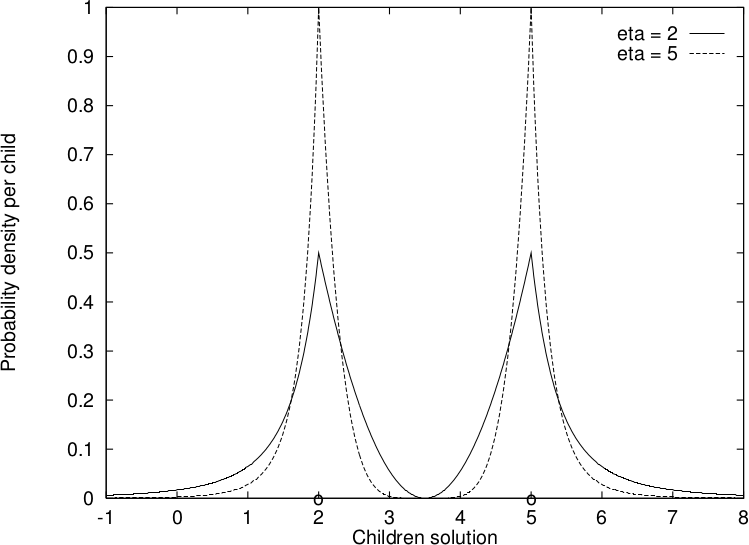
\includegraphics{img/appendixC/sbx.png}
        }
        \vspace{-0.25cm}
        \caption{\tiny~Ilustración que describe el proceso de Cruzamiento.~\textit{Adaptado de:}~\cite{stackoverflow_crossover_index_2019}}%
        \label{fig:tournament_selection}
    \end{figure}
\end{frame}

\begin{frame}{Anexo \thesection~: Mutación}%
    \vspace{-0.15cm}
    \begin{figure}[H]
        \centering
        \adjustbox{max width=\textwidth, max height=0.7\textheight}{%
            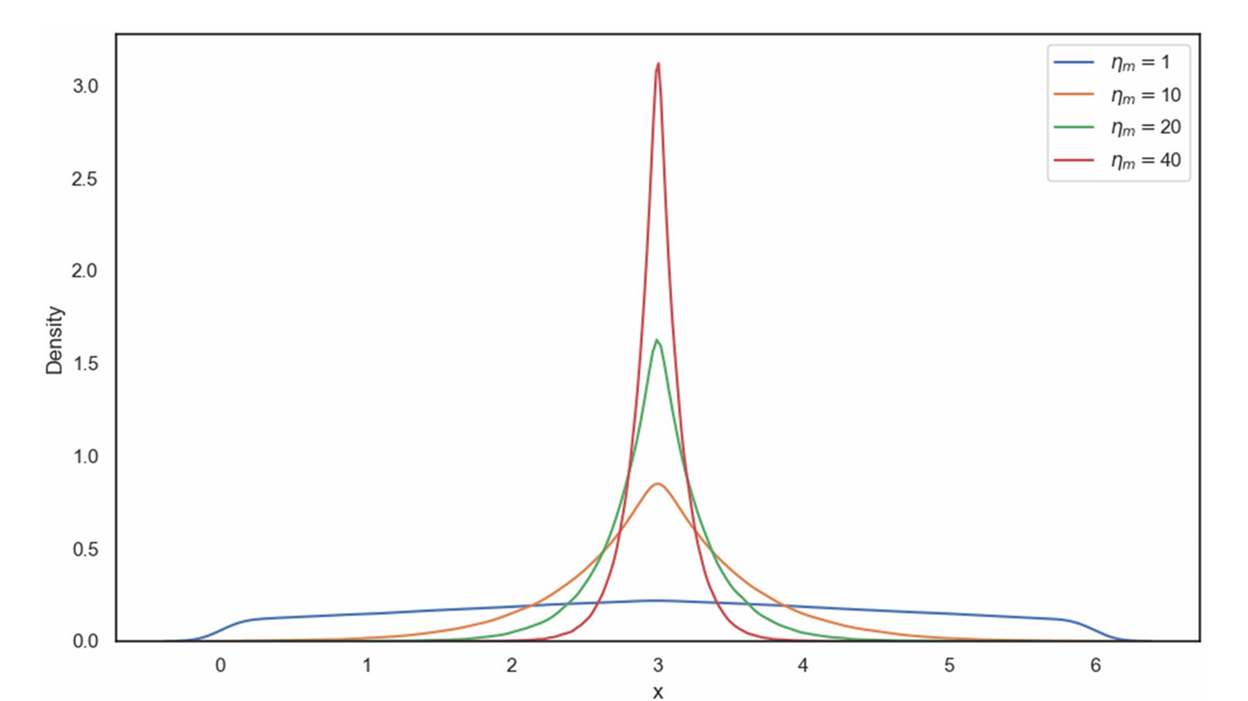
\includegraphics{img/appendixC/polynomialMutation.png}
        }
        \vspace{-0.25cm}
        \caption{\tiny~Ilustración que describe el proceso de Mutación.~\textit{Adaptado de:}~\cite{CarlesBou2023}}%
        \label{fig:tournament_selection}
    \end{figure}
\end{frame}